% =============================================
% ==          sections/methods.tex           ==
% =============================================
\section{Methodology}\label{sec:methods}

This section details the formal framework of our study, the core mechanics of the evaluated algorithms, which includes algorithms centered on MAPPO as well as other algorithms used for comparison.

\subsection{Preliminaries: The Dec-POMDP Framework}

The essence of multi-agent cooperative tasks lies in the collective effort of multiple agents to achieve a common objective through dynamic decision-making and behavioral collaboration within a partially observable environment. To fundamentally comprehend this process, it is imperative to first examine the Decentralized Partially Observable Markov Decision Process (Dec-POMDP)~\cite{oliehoekConciseIntroductionDecentralized2016}, which enables a precise characterization of the limitations of agents' local observations, the dynamics of environmental states, and the collaborative interdependencies among agents. This also constitutes the core theoretical foundation for research in Multi-Agent Reinforcement Learning (MARL).
A Dec-POMDP is formally defined by the tuple  $\langle \mathcal{S}, \mathcal{A}, P, R, \mathcal{Z}, O, n, \gamma \rangle$, where:
\begin{itemize}
    \item $s \in \mathcal{S}$ is the true global state of the environment.For instance, in the context of StarCraft II cooperative tasks, a state $s \in \mathcal{S}$ encompasses not only individual agent attributes such as position and energy levels but also environmental information like the distribution of enemy units. 
    \item $a \in \mathcal{A}^n$ is the joint action, composed of individual actions $a_i \in \mathcal{A}$ from each of the $n$ agents.
    \item $P(s'|s, a): \mathcal{S} \times \mathcal{A}^n \times \mathcal{S} \to [0, 1]$ is the state transition function.
    \item $R(s, a): \mathcal{S} \times \mathcal{A}^n \to \mathbb{R}$ is the shared reward function for all agents.
    \item $z \in \mathcal{Z}$ is a joint observation. Each agent $i$ receives a local observation $z_i$ according to the observation function $O(s, i)$.
    \item $O(s, i): \mathcal{S} \times \{1, \ldots, n\} \to \mathcal{Z}$ defines the probability of each agent receiving a particular observation given the global state.
    \item $n$ is the number of agents.
    \item $\gamma \in [0, 1)$ is the discount factor.
\end{itemize}
Collectively, these components transform the multi-agent cooperation problem into an optimization challenge: finding the optimal joint policy $\pi^* = (\pi_1^*, \pi_2^*, \ldots , \pi_n^*)$ that maximizes the expected cumulative reward,
\begin{equation} 
     J (\pi) = \mathbb{E}_{\pi} \left[ \sum_{t=0}^{\infty} \gamma^t R (s_t, a_t) \right],
\end{equation}
under the constraints of partial observability. This provides a robust theoretical basis for the subsequent design and performance evaluation of our proposed MAPPO algorithm and its counterparts.

\subsection{MAPPO Algorithm Architecture and Objective Functions}

Multi-Agent Proximal Policy Optimization (MAPPO) represents a critical extension of the single-agent PPO algorithm to the Centralized Training with Decentralized Execution (CTDE) framework~\cite{yuSurprisingEffectivenessPPO2022}. Its core design philosophy is to leverage an architecture of independent Actors and a shared, centralized Critic, thereby balancing the flexibility of decentralized execution with the global optimization capabilities of centralized training.

\subsubsection*{Network Architecture Design}
The network architecture of MAPPO is explicitly partitioned into an ``execution layer'' and a ``training layer''.

\paragraph{Actor Network (Core of the Execution Layer)}
Each agent $i$ is equipped with an independent actor network, denoted as:
$\pi_{\theta_i}(a_i|o_i)$
where $\theta_i$ represents the learnable parameters of this actor. The input to the actor network is the local observation $o_i$ of agent $i$, and its output is the action probability distribution for that agent. During the decentralized execution phase, each agent makes decisions independently based solely on its own actor network and local observation, eliminating the need for real-time information exchange with other agents. In terms of network structure, the MAPPO Actor typically employs a deep learning architecture consisting of fully connected layers with ReLU activation functions. The input layer's dimensionality matches the local observation space $\Omega_i$, followed by 2--3 hidden layers to introduce non-linear transformations. The output layer utilizes a Softmax function to convert neural outputs into a valid action probability distribution.

From the perspective of the actor's objective function, the policy update is constrained by clipping the probability ratio of the new and old policies, $r_t(\theta_i)$, within the interval $[1-\epsilon, 1+\epsilon]$. The mathematical expression for this clipped objective is:
\begin{equation}
    L_{\text{clip}}(\theta_i) = \mathbb{E}_t \left[ \min \left( r_t(\theta_i) \hat{A}_t,\, \text{clip}\left( r_t(\theta_i),\, 1-\epsilon,\, 1+\epsilon \right) \hat{A}_t \right) \right].
\end{equation}
The clipped loss $L_{\text{clip}}(\theta_i)$ is calculated independently for each agent's actor network. The total actor loss to be optimized is the sum of all individual actor losses:
\begin{equation}
    L_{\text{Actor}} = \sum_{i=1}^n L_{\text{clip}}(\theta_i).
\end{equation}
This structure effectively fits the complex mapping between local observations and action decisions, thereby satisfying the demand for low communication overhead in practical scenarios~\cite{yuSurprisingEffectivenessPPO2022}.

\paragraph{Critic Network (Core of the Training Layer)}
All agents share a single, centralized critic network, denoted as:$V_{\phi}(s)$,
where $\phi$ represents the learnable parameters of the critic. The input to the critic network is the global state $s$, and its output is the state-value estimate, which evaluates the expected long-term cumulative reward of the system under the current policy. The architecture of the centralized critic is similar to that of the actor, but its input dimensionality matches the global state space $S$, and its output layer consists of a single neuron without a Softmax activation. By leveraging global state information, the critic can more accurately assess the contribution of the joint action to the overall task objective.

The critic's objective function focuses on minimizing the Mean Squared Error (MSE) between the state-value estimate and a target value. Its mathematical expression is:
\begin{equation}
    L\left( {\phi} \right) = \mathbb{E}_t\left[ \left( V_{\phi}\left( s_t \right) - Y_t \right)^2 \right].
\end{equation}
Here, $Y_t$ is the target value, commonly calculated using the Temporal Difference (TD) target:
\begin{equation}
    Y_t = R(s_t, a_t) + \gamma V_{\phi^{\text{old}}}(s_{t+1}),
\end{equation}
where $V_{\phi^{\text{old}}}(s_{t+1})$ is the value estimate from a target critic network whose parameters are periodically synchronized and fixed~\cite{yuSurprisingEffectivenessPPO2022}. Since all agents share the critic network, the computation of $L(\phi)$ is based on the global state $s_t$ and the joint action $a_t$. This allows for the integration of behavioral information from all agents, providing high-quality gradient signals to each actor and effectively addressing the challenge of credit assignment arising from partial observability.

\subsection{Baseline Algorithms}

To conduct a comprehensive performance evaluation of MAPPO, this study provides a detailed explication of the core mechanisms, network architectures, and optimization logic of several baseline algorithms (QMIX, OW-QMIX, and IPPO). This serves to establish a clear algorithmic context for the subsequent experimental comparisons.

\subsubsection{QMIX:~Monotonic Value Function Decomposition}

As a canonical example of Monotonic Value Function Decomposition algorithms, the core innovation of QMIX lies in its use of a monotonic mixing network to transform individual agent Q-values into a joint Q-value. This design simultaneously satisfies the ``centralized trainin'' requirement of the CTDE framework while supporting ``decentralized execution''.

As shown in the figure~\ref{fig:QMIX architecture}, the architecture of QMIX is composed of two primary components: agent networks and a mixing network.
\begin{figure*}[htbp]
    \centering %
    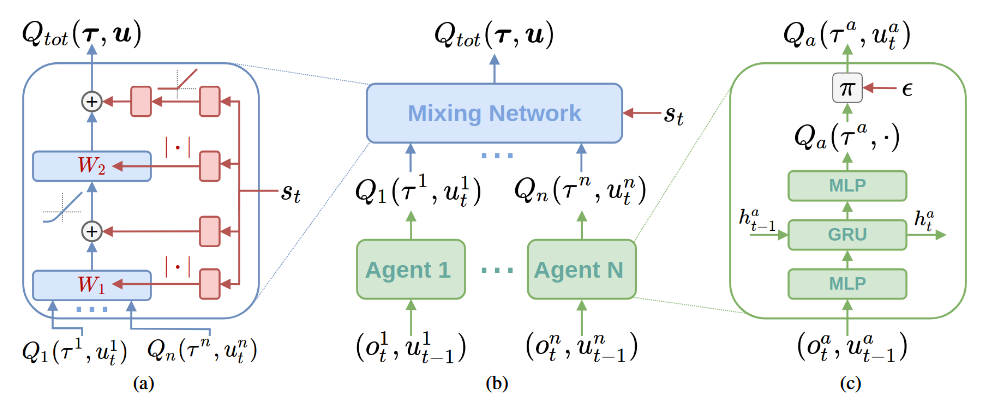
\includegraphics[width=0.8\textwidth]{QMIX architecture.png}
    \caption{
        (a) Structure of the mixing network. Highlighted in red are the hypernetworks, which generate the weights and biases for the mixing network layers (marked in blue). 
        (b) Overall architecture of the QMIX framework. 
        (c) Architectural design of the agent network. 
        Adapted from Fig.~2 in~\cite{rashidQMIXMonotonicValue2018}
    }\label{fig:QMIX architecture}
\end{figure*}

\paragraph{Agent Networks}
Each agent $i$ possesses an independent Q-network:
$
Q_i(o_i, a_i; \theta_i).
$
The network takes the local observation $o_i$ and action $a_i$ as input and outputs the individual Q-value, $Q_i(o_i, a_i)$, which represents the estimated value of agent $i$ taking action $a_i$ given its local observation. The structure of the QMIX agent network is analogous to that of the MAPPO Actor, employing fully connected layers with ReLU activation functions, and its output layer is a single real-valued scalar.

\paragraph{Mixing Network}
All agents share a single mixing network~\cite{rashidQMIXMonotonicValue2018}, denoted as $g(\cdot; \phi)$. This network takes the set of all individual Q-values, $\{Q_1, Q_2, \dots, Q_n\}$, along with the global state $s$ as input, and outputs the joint Q-value:
\begin{equation}
    Q_{\text{tot}}(s, a) = g(Q_1(o_1, a_1), \dots, Q_n(o_n, a_n); s; \phi).
\end{equation}
A critical constraint (\refeq{eq:partial_derivative_condition}) imposed on the mixing network is monotonicity, which ensures that for all agents $i$.
This guarantees a monotonically increasing relationship between the global joint Q-value, $Q_{\text{tot}}$, and each individual agent's Q-value, $Q_i$. Consequently, the greedy selection of actions at the individual level naturally corresponds to the greedy selection of the joint action at the global level.

Furthermore, a key optimization objective for QMIX is to minimize the Mean Squared Error between the joint Q-value and a target Q-value. This is formulated~\cite{rashidQMIXMonotonicValue2018} as the loss function:
\begin{equation}
    L_{\text{QMIX}} = \mathbb{E}_t\left[ (Q_{\text{tot}}(s_t, a_t; \theta, \phi) - Y_t^{\text{QMIX}})^2 \right],
\end{equation}
where $\theta = (\theta_1, \dots, \theta_n)$ represents the parameters of all agent networks, and $\phi$ denotes the parameters of the mixing network.

During the training process, QMIX utilizes centralized data to optimize both the mixing and agent networks. In the execution phase, however, each agent acts decentrally by selecting the action that maximizes its local Q-value, without requiring any global information:
\begin{equation}
    a_i^* = \arg\max_{a_i \in A_i} Q_i(o_i, a_i).
\end{equation}

In summary, this design, which enforces non-negativity on the mixing network's weights, not only simplifies the optimization challenge but also ensures the theoretical soundness of the value function decomposition.

\subsubsection{OW-QMIX:~An Extended QMIX with Optimistic Weighting}

OW-QMIX (Optimistically-Weighted QMIX) is an extension of the QMIX algorithm. Its primary enhancement is the introduction of a weighted projection mechanism, which assigns differential weights to various joint actions. This prioritizes the optimization of value estimates for superior joint actions, thereby aiming to overcome the representational limitations inherent in QMIX's monotonic value function decomposition.

In terms of its core philosophy and network architecture, OW-QMIX largely aligns with QMIX, similarly incorporating ``agent network'' and a ``mixing network''. However, it introduces two critical new components: an unconstrained joint value function, denoted as $\hat{Q}^*$, and an optimistic weighting function.

The agent networks in OW-QMIX function identically to those in QMIX.\@ Each agent $i$ employs an independent Q-network, $Q_i(o_i, a_i; \theta_i)$, to output an individual Q-value, with a network structure based on fully connected layers and ReLU activation functions. The mixing network builds upon QMIX's monotonic foundation, but its input is expanded to include not only the individual Q-values and the global state $s$, but also agent trajectory information, such as observation sequences ($o_{i,1:t}$) and action sequences ($a_{i,1:t}$). This is processed through a temporal feature encoding module to capture the long-term dependencies between behavior and environmental dynamics.

The newly introduced unconstrained value function, $\hat{Q}^*$, utilizes a mixing network architecture that is free from the monotonicity constraint. It directly takes the global state, joint action, and trajectory information as input to approximate the true joint value function. The weights of its mixing network are not required to be non-negative, enabling it to model more complex multi-agent interactions. The optimistic weighting function assigns weights to joint actions based on the condition:
\[
Q_{\text{tot}}(s_t, a_t, o_{1:t}, a_{1:t}) < Y_t^{\text{OWQMIX}}.
\]
When this condition is met, a weight of 1 is assigned, thereby emphasizing the estimation accuracy for potentially optimal actions.

The optimization objective of OW-QMIX remains centered on minimizing the joint Q-value estimation error, but its loss function incorporates the weighting mechanism and the expanded state information:
\begin{multline}
    L_{\text{OWQMIX}} = \mathbb{E}_t\Big[ w(s_t, a_t) \cdot \\
    \left(Q_{\text{tot}}(s_t, a_t, o_{1:t}, a_{1:t}; \theta, \phi) - Y_t^{\text{OWQMIX}}\right)^{2} \Big].
\end{multline}
The target value, $Y_t^{\text{OWQMIX}}$, is defined as:

\begin{equation}
\begin{split}
    Y_t^{\text{OWQMIX}} ={}& R(s_t, a_t) + \gamma \hat{Q}^*\big(s_{t+1}, \tau_{t+1}, \\
    & \arg\max_{u'} Q_{\text{tot}}(s_{t+1}, \tau_{t+1}, u')\big),
\end{split}
\end{equation}
where $\tau$ represents the set of agent trajectories.

During training, the agent networks, the mixing network, and the $\hat{Q}^*$ network are optimized simultaneously, with parameters updated using centrally stored, multi-dimensional data. The execution phase is identical to that of QMIX, employing a decentralized decision-making model where each agent selects its action based on its own individual Q-value~\cite{rashidWeightedQMIXExpanding2020}.

\subsubsection{IPPO:~Independent PPO}

The core philosophy of IPPO (Independent PPO) is to treat a multi-agent task as a concurrent collection of independent single-agent tasks. Under this paradigm, each agent executes its own PPO algorithm, viewing the behavior of all other agents as part of the environment's dynamics. Each agent $i$ is equipped with an independent actor network, $\pi_{\theta_i}(a_i|o_i)$, and an independent critic network, $V_{\phi_i}(o_i)$. The parameters of these networks are entirely separate for each agent, with no sharing or coordination mechanisms.

In terms of network architecture, there is a significant difference between IPPO and MAPPO, particularly concerning the critic network. In IPPO, each agent $i$ possesses its own actor and critic networks whose parameters are mutually independent. Specifically, the structure of IPPO's actor network,
$
\pi_{\theta_i}(a_i|o_i)
$
is identical to that of MAPPO's, taking a local observation $o_i$ as input and outputting an action probability distribution, which is then optimized using PPO's Clipped Surrogate Objective.

However, the critic network in IPPO diverges from that in MAPPO. IPPO's critic is decentralized, taking only the local observation $o_i$ as input and producing a local state-value estimate:
$
V_{\phi_i}(o_i)
$
Its loss function is defined as:

\begin{equation}
    L_{\text{Critic},i} = \mathbb{E}_t\left[ (V_{\phi_i}(o_{i,t}) - Y_{i,t})^2 \right],
\end{equation}
where $Y_{i,t}$ is the TD target computed solely based on local observations, without incorporating any global information~\cite{wittIndependentLearningAll2020}.

A major drawback of this approach is the issue of non-stationarity. On account of ignoring the policy shifts of other agents, the ``effective environment'' for any given agent is constantly changing. As other agents update their policies, an agent's own policy can become obsolete, making it difficult for the system to converge to a stable and cooperative joint policy.

\subsection{Evaluation Benchmarks in MARL}
The empirical validation of MARL algorithms heavily relies on robust and challenging benchmarks. While early research utilized simpler grid-world environments, the field has increasingly adopted more complex domains. The StarCraft II Multi-Agent Challenge (SMAC)~\cite{samvelyanStarCraftMultiAgentChallenge2019} has emerged as a recognized standard. Its diverse set of micromanagement scenarios, characterized by partial observability, high-dimensional state-action spaces, and delayed rewards, provides a fertile ground for rigorously testing the limits of cooperative MARL algorithms. To ensure a fair and reproducible comparison, we leverage the XuanCe library~\cite{liuXuanCeComprehensiveUnified2023}, which offers standardized implementations of the algorithms under investigation.
